\begin{enumerate}[label=\thesubsection.\arabic*.,ref=\thesubsection.\theenumi]
\numberwithin{equation}{enumi}
\item Sketch the polar plot of 
\begin{align}
    G(s) = \frac{1}{(s^2)(s+1)(s+2)}. 
    \label{eq:ee18btech11028_1}
\end{align}
%
\solution
Substituting $s = \j\omega$ in      \eqref{eq:ee18btech11028_1},

Now the magnitude will be
\begin{align}
   r &=  |G(\j\omega)| = \frac{1}{(\omega^2)(\sqrt{1 + \omega^2})(\sqrt{1+4\omega^2})}
    \label{eq:ee18btech11028_2}
\\
\theta &=\angle G(\j\omega)  = - \tan^{-1}(0) - \tan^{-1}(\omega) - \tan^{-1}(2\omega)
\\
     &= 180\degree - \tan^{-1}(\omega) - \tan^{-1}(2\omega)
    \label{eq:ee18btech11028_3}
\end{align}

The polar plot is the $\brak{r,\theta}$ plot for $\omega \in \brak{0,\infty}$.
The following python code generates  the polar plot in Fig. \ref{fig:ee18btech11028_fig1}
\begin{lstlisting}
    codes/ee18btech11028.py
\end{lstlisting}
\begin{figure}[!h]
\centering
    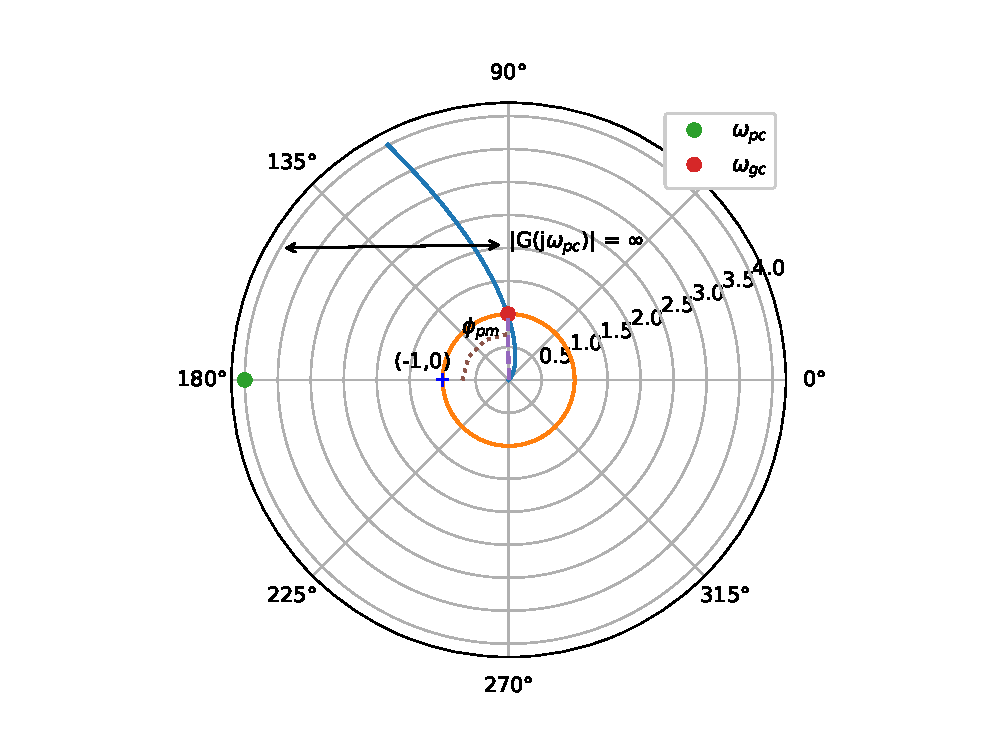
\includegraphics[width=\columnwidth]{./figs/ee18btech11028.eps}
  \caption{}
  \label{fig:ee18btech11028_fig1}
\end{figure}
The location of $\brak{-1,0}$ with respect to the polar plot provides information regarding the stability of the system.  
\begin{itemize}
    
    \item If  \brak{–1,0} is not enclosed, then it is stable.
    \item If \brak{–1,0} is enclosed by polar plot then it is unstable. 
    \item If \brak{–1,0} is on the polar plot then it is marginally stable
    
    
\end{itemize}
In Fig. \ref{fig:ee18btech11028_fig1},  the point \brak{-1,0} is enclosed by the polar plot,
which implies system is not stable.  The polar plot also provides info on the GM and PM, which can then be used for determining the stability of the system.

\begin{itemize}
    \item If the $GM > 1 \cap PM > 0$,  then the control system is \textbf{stable}.
    \item If the $GM = 1\cap PM =0 $,  then the control system is  \textbf{marginally stable}.
    \item If the $GM < 1\cup  PM < 0$ , then the control system is \textbf{unstable}.
\end{itemize}

Therefore, our system is unstable $\because GM < 1\cap  PM < 0$.



\end{enumerate}
